\documentclass{article}
\usepackage{amsmath}
\usepackage{graphicx} 
\usepackage{booktabs}



\title{Mathematics for Economics}
\author{Lajos Galambos}
\date{August 2024}

\begin{document}

\maketitle

\section{Introduction}
This is a note created for BA/MA level Mathematics for Economic Science based on the book of Knut Sydsæter and Peter Hammond: Essenatial Mathematics for Economic Analysis. This is part of my preparation for PhD application, and in general, to revise everything that is necessary to become an economist. 

\section{Algebra}
Natural Numbers – Integers – Rational Numbers – Irrational Numbers [infinite non periodic decimals] – Real Numbers

\subsection{Integer Powers}
\begin{equation}
  a^n = a \times a \times \ldots \times a \quad \text{(n times)}
\end{equation}

\begin{equation}
  a^0 = 1 \quad \text{for } a \neq 0
\end{equation}

\begin{equation}
  a^{-n} = \frac{1}{a^n}
\end{equation}

\subsection{Properties Powers}
\begin{equation}
  a^r \times a^s = a^{(r+s)}
\end{equation}

\begin{equation}
  (a^r)^s = a^{(r \times s)}
\end{equation}

\begin{equation}
  \frac{a^r}{a^s} = a^{(r - s)}
\end{equation}

\begin{equation}
  (ab)^r = a^r \times b^r
\end{equation}

\begin{equation}
  \left(\frac{a}{b}\right)^r = \frac{a^r}{b^r}
\end{equation}

\begin{equation}
  (abcde)^r = a^r \times b^r \times c^r \times d^r \times e^r
\end{equation}

\begin{equation}
  (a+b)^r \neq (a \times b)^r
\end{equation}

\subsection{Rules of Algebra}
In algebraic expressions, polynomials are defined by: \textbf{numerical coefficients}, and \textbf{terms of same type}. We can use \textbf{factoring} to make expressions more convenient to read. \\

Quadratic identities:
\begin{equation}
  (a+b)^2 = a^2 + 2ab + b^2
\end{equation}

\begin{equation}
  (a-b)^2 = a^2 - 2ab + b^2
\end{equation}

\begin{equation}
 (a+b)(a-b) = a^2 - b^2
\end{equation}

\subsection{Fractions}
Rules of fractions: 

\begin{equation}
 \frac{a\times c}{b\times c} = \frac{a}{b} \quad \text{for } b \neq 0 \text{ and } c \neq 0
\end{equation}

\begin{equation}
 \frac{-a}{-b} = \frac{a}{b} 
\end{equation}

\begin{equation}
 -\frac{a}{b} = \frac{-a}{b} 
\end{equation}

\begin{equation}
 \frac{a}{c} + \frac{b}{c} = \frac{a + b}{c} 
\end{equation}

\begin{equation}
 \frac{a}{b} + \frac{c}{d} = \frac{ad + cd}{bd} 
\end{equation} \\

LCD is a technique, finding the Least Common Denominator. It is used in especially the case of equation (18). \\

\begin{equation}
 a + \frac{b}{c} = \frac{ac + b}{c} 
\end{equation}

\begin{equation}
 a \times \frac{b}{c} = \frac{ab}{c} 
\end{equation}

\begin{equation}
 \frac{a}{b} \times \frac{c}{d} = \frac{ac}{bd} 
\end{equation}

\begin{equation}
 \frac{a}{b} \div \frac{c}{d} = \frac{a}{b} \times \frac{d}{c} 
\end{equation}

\subsection{Fractional Powers}
Powers can be written in a fractional form (if in the power we have rational numbers). Those are square roots. 

\begin{equation}
  a^{\frac{1}{2}} = \sqrt{a} \quad \text{valid if } a \geq 0
\end{equation}

\begin{equation}
 \sqrt{a} \times \sqrt{b} = \sqrt{ab}
\end{equation}

\begin{equation}
 \sqrt{\frac{a}{b}} = \frac{\sqrt{a}}{\sqrt{b}}
\end{equation}

\begin{equation}
 \sqrt{a} + \sqrt{b} \neq \sqrt{a} + \sqrt{b} \quad \text{(in general)}
\end{equation}

\begin{equation}
 a^{\frac{1}{n}} = \sqrt[n]{a} 
\end{equation}

\begin{equation}
 a^{\frac{p}{q}} = (\sqrt[q]{a})^p = \sqrt[q]{a}^p  \quad\text{(p an integer, q a natural number)}
\end{equation}

\subsection{Inequalities}

(1) If the two sides of an inequality are multiplied by a positive number, the direction of the inequality is preserved.
(2) If the two sides of an inequality are multiplied by a negative number, the direction of the inequality is reversed.

\begin{equation}
 \text{If } a > 0 \text{ and } b > 0, \text{ then } a + b > 0 \text{ and } a \times b > 0
\end{equation}

\begin{equation}
 \text{If } a > b, \text{ then } a - b > 0
\end{equation}

\begin{equation}
 \text{If } a \geq b, \text{ then } a - b \geq 0
\end{equation}

\begin{align}
 \text{If } a > b \text{ and } b > c, \text{ then } a > c \\
 \text{If } a > b \text{ and } c > 0, \text{ then } a \cdot c > b \cdot c \\
 \text{If } a > b \text{ and } c < 0, \text{ then } a \cdot c < b \cdot c \\
 \text{If } a > b \text{ and } c > d, \text{ then } a + c > b + d
\end{align} 

\begin{figure}[h]
\centering
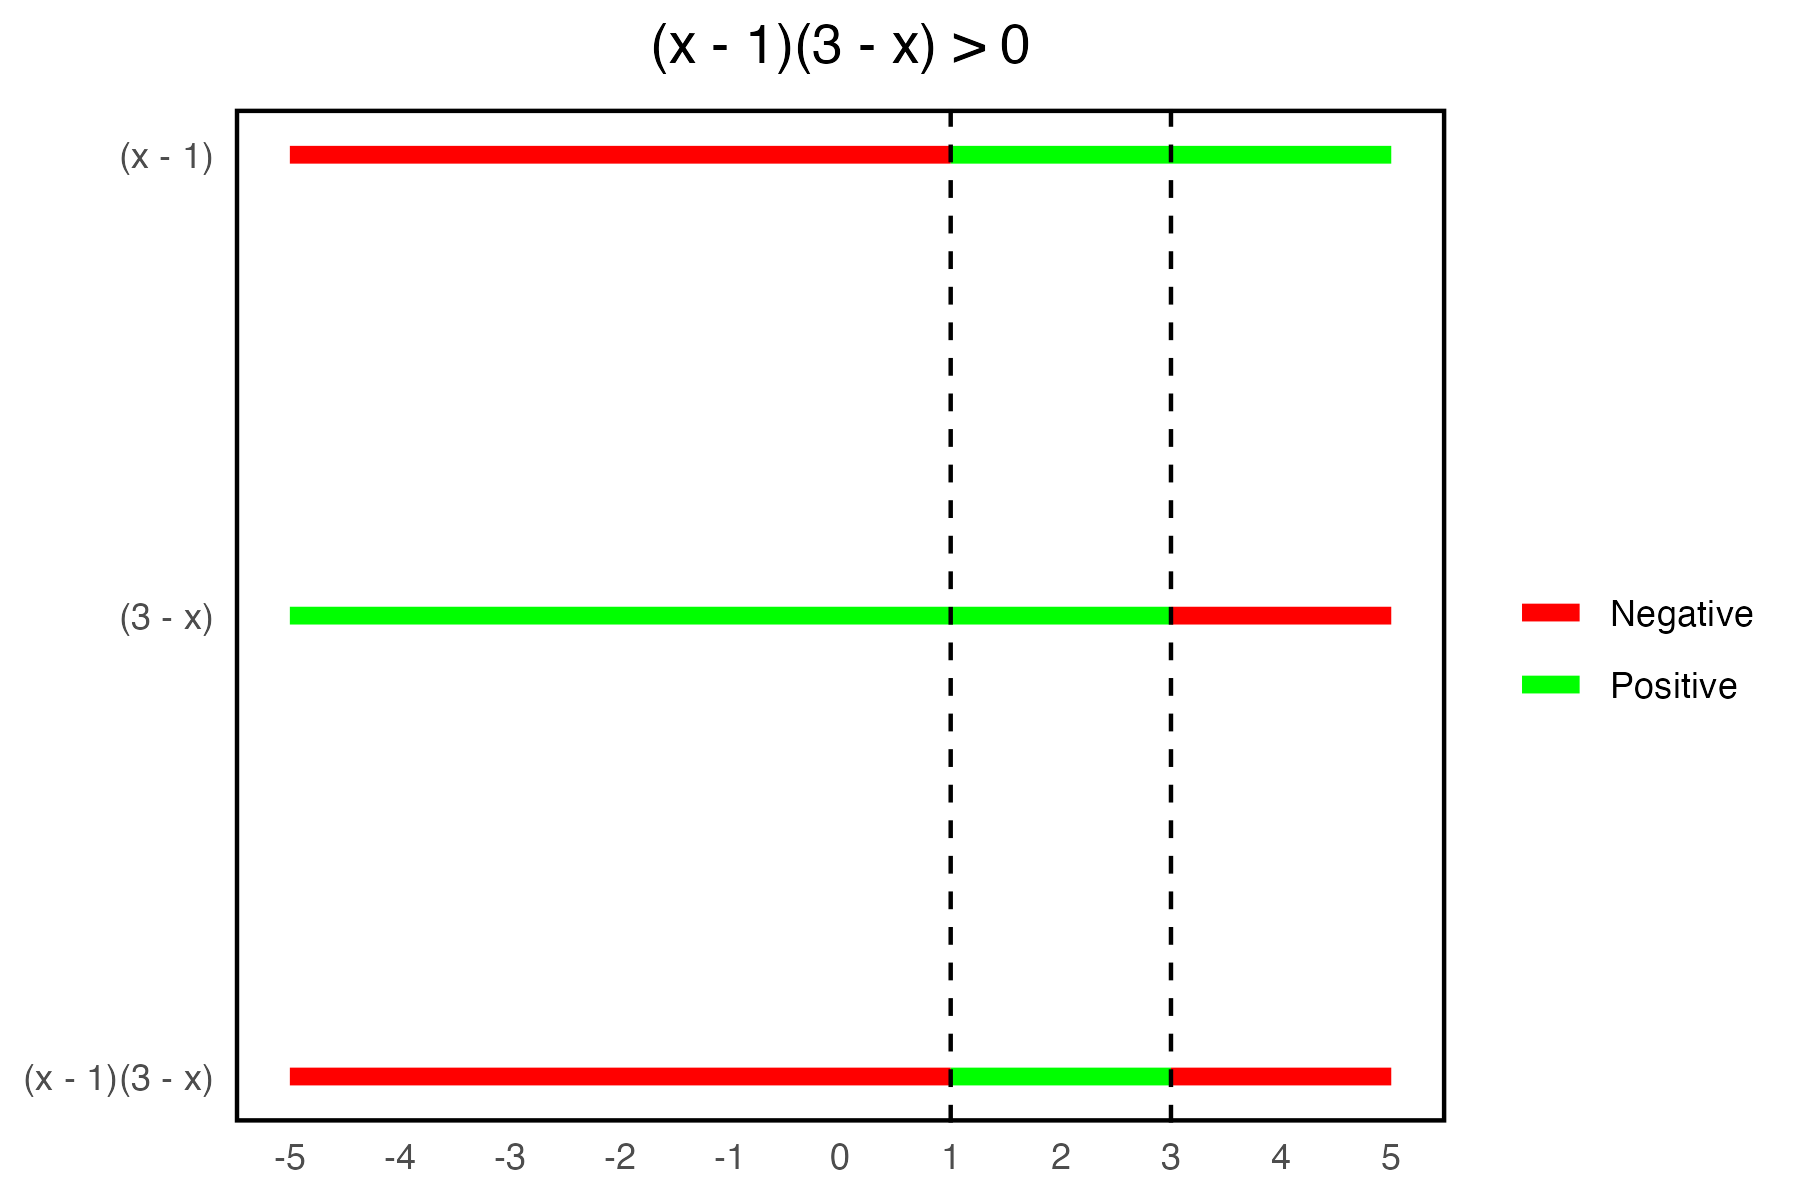
\includegraphics[width=0.8\textwidth]{Sign_Diagram.png}
\caption{Sign Diagram}
\end{figure}

Two inequalities that are valid simultaneously are often written as a \textbf{double inequality}. If, for example, \(a \leq z\) and moreover \(z < b\), it is natural to write \(a \leq z < b\). \\

\subsection{Intervals}
\begin{table}[h]
\centering
\caption{Notation of Intervals} 
\begin{tabular}{l|l|l}
\hline
Notation & Name & The interval consists of all x satisfying: \\
\hline
(a, b) & The open interval from a to b. & $a < x < b$ \\
\hline
[a, b] & The closed interval from a to b. & $a \leq x \leq b$ \\
\hline
(a, b] & A half-open interval from a to b. & $a < x \leq b$ \\
\hline
[a, b) & A half-open interval from a to b. & $a \leq x < b$ \\
\hline
\end{tabular}
\end{table}

\[ [a, \infty) = \{ x \mid x \geq a \} \]
\[ (-\infty, b) = \{ x \mid x < b \} \] \\

The \textbf{absolute value} of "a" is defined as the distance of "a" from 0 on the number line; expressed as follows: 

\begin{equation}
|a| = 
\begin{cases} 
a & \text{if } a \geq 0 \\
-a & \text{if } a < 0 
\end{cases}
\end{equation}

\begin{equation}
|x_1 - x_2| = |x_2 - x_1| = \text{distance between } x_1 \text{ and } x_2 \text{ on the number line}
\end{equation}

\begin{figure}[h]
\centering
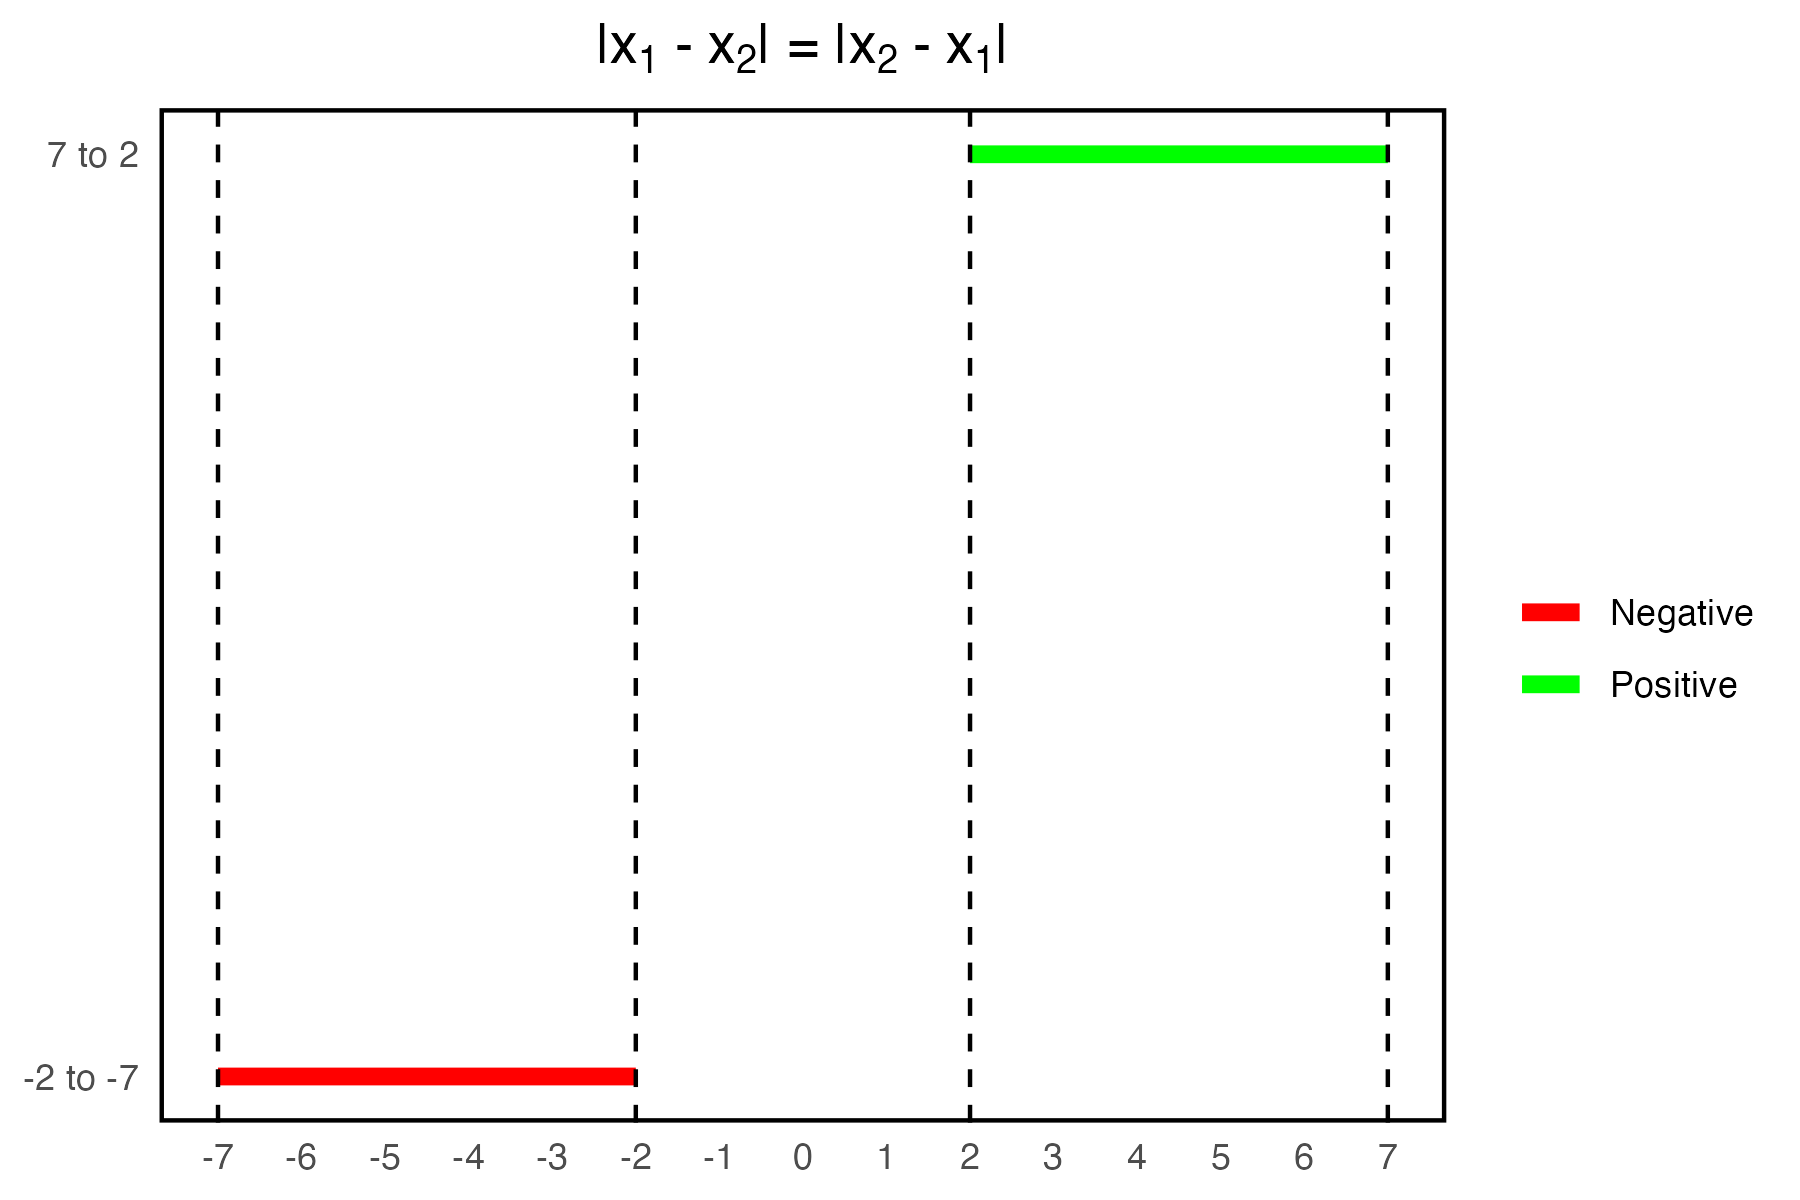
\includegraphics[width=0.8\textwidth]{Distance_Diagram.png}
\caption{Distance on the Number Line is 5 in both cases}
\label{fig:distance_diagram}
\end{figure}

\section{Equations}
\subsection{Simple Linear Equations}

Basic rule: to get equivalent equations, do the following on both sides of the equality sign: 
\begin{itemize}
\item[(A)] add (or subtract) the same number,
\item[(B)] multiply (or divide) by the same number $\neq 0$.
\end{itemize}

\textbf{\textit{Example:}}

Take an example from economics: A firm manufactures a commodity that costs 20 Dollars per unit to produce. In addition, the firm has fixed costs of 2000 Dollars. Each unit is sold for 75 Dollars. How many units must be sold if the firm is to meet a profit target of 14500 Dollars ?

\begin{align*}
75Q - (20Q + 2000) &= 14500 \\
55Q - 2000 &= 14500 \\
55Q &= 16500 \\
Q &= \frac{16500}{55} \\
Q &= 300
\end{align*}

\begin{figure}[h]
\centering
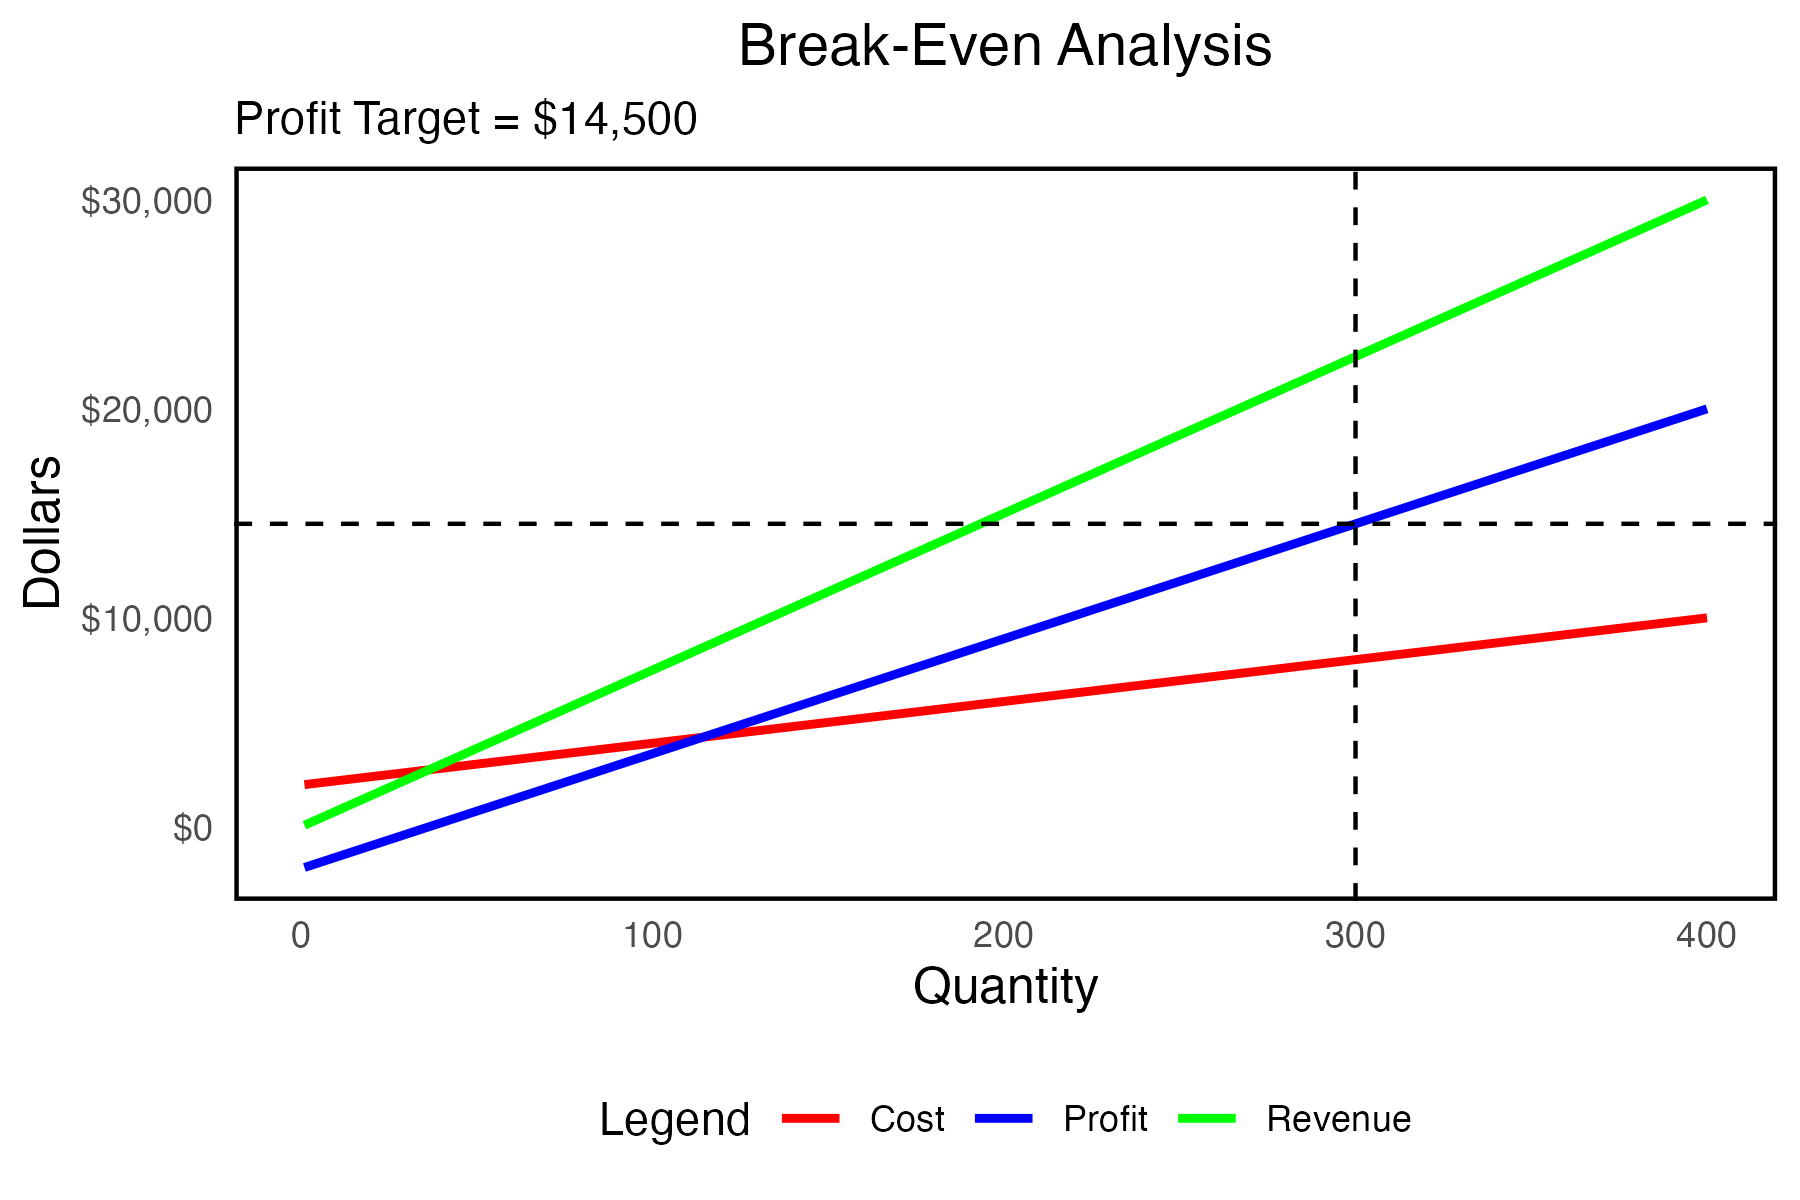
\includegraphics[width=0.8\textwidth]{Profit_Break_Even.png}
\caption{Solving for Q gives the Break-Even point of production}
\label{fig:distance_diagram}
\end{figure}

\subsection{Equations with Parameters}

The general equation (38) describes a whole class of linear equations where x and y are the variables. The letters a and b are called parameters, and they take on different values:

\begin{equation}
y = ax + b
\end{equation}

in economics the term of the\textit{ national income identity}: 

\begin{equation}
Y = C + \bar{I}\footnote{In economics, we often use a bar over a symbol to indicate that it is fixed. An alternative notation is to use the superscript 0, e.g. Y = C +I$^0$, or the subscript 0, e.g. Y = C +I$_0$.}
\end{equation}

Economists usually call the two equations in (39) the structural form of the model, whereas in the following part is the reduced form that expresses \textbf{endogenous variables} as functions of \textbf{exogenous variables}:

\begin{align*}
Y &= C + \bar{I} \\
C &= a + bY
\end{align*}

\begin{align*}
Y - bY &= a + \bar{I} \\
Y(1 - b) &= a + \bar{I} \\
Y &= \frac{a}{1 - b} + \frac{1}{1 - b} \bar{I} \\
\end{align*}

\textbf{Reminder: } the whole point of solving for certain variables in parametric expressions is to isolate certain variables in a way that they are only defined by other variables (not themselves). Put it bluntly, the variable that I am solving for should only be on \textbf{one side of the equation}. We might want to \textbf{use factoring} on the way to solve for certain variables. 

\subsection{Quadratic Equations}

Also called second-degree, the general form looks like: 
\begin{equation}
ax^2 + bx + c = 0 \quad (a \neq 0)
\end{equation}

where a, b, and c are given constants, and x is the unknown. After dividing by (a) we get: 
\begin{align*}
x^2 + \left(\frac{b}{a}\right)x + \frac{c}{a} = 0
\end{align*}
If we add parameters to the quotients, we arrive to the a general form. If p = b/a and q = c/a, the equation is:

\begin{equation}
x^2 + px + q = 0
\end{equation}
\textbf{There can be two common cases for parametric equation 41:}

\begin{itemize}
\item \textbf{If $q = 0$} (there is no constant term), the equation reduces to 
\begin{align*}
x^2 + px &= 0 \\
x(x + p) &= 0 \\
x &= 0 \text{ or } x = -p
\end{align*}

\item  \textbf{If $p = 0$} (there is no term involving x), the equation (41) reduces to
\begin{align*}
x^2 + q &= 0 \\
x^2 &= -q \\
x &= \pm \sqrt{-q} \quad (q \leq 0)
\end{align*}
\end{itemize}
\textbf{The general quadratic formula: }
\begin{equation}
x = \frac{-b \pm \sqrt{b^2 - 4ac}}{2a}
\end{equation}
\text{if and only if } $b^2 - 4ac \geq 0$ \text{ and } $a \neq 0$. The solutions are often called the roots of the equation. \textbf{ It goes backwards too:} \text{if } $x_1$ \text{ and } $x_2$ \text{ are the solutions of } $ax^2 + bx + c = 0$, it can be re-written:
\begin{equation}
ax^2 + bx + c = a(x - x_1)(x - x_2)
\end{equation}
Which comes from the rules of powers (previous chapter):
\begin{align*}
(a+b)^2 = (a+b)(a+b)
\end{align*}
\subsection{Linear Equations in Two Unknowns}
We need to find the values of x and y that satisfy both equations. \\

\textbf{Example:}
\begin{align*}
2x + 3y &= 18 \\
3x - 4y &= -7
\end{align*}

\textbf{Method 1}: solve one of the equations for one of the variables \textbf{in terms of the other}; then substitute the result into the other equation. This leaves only one equation in one unknown, which is easily solved.
\begin{align*}
2x + 3y &= 18 \\
x &= \frac{18 - 3y}{2} \quad \text{(1)}
\end{align*}

Substitute \text{(1)} into the second equation:

\begin{align*}
3\left(\frac{18 - 3y}{2}\right) - 4y &= -7
\end{align*}

\textbf{Method 2}: is based on eliminating one of the variables by adding or subtracting a multiple of one equation from the other.

\begin{align*}
8x + 12y &= 72 \quad \text{(1)} \\
9x - 12y &= -21 \quad \text{(2)}
\end{align*}

Add \text{(1)} and \text{(2)}:

\begin{align*}
(8x + 12y) + (9x - 12y) &= 72 + (-21) \\
17x &= 51
\end{align*}

\subsection{Non Linear Equations (when = 0)}

Non linear equations are used in economics especially for doing optimization problems. Solving for 0 is a simple task. First, recall that a product of two or more factors is 0 if and only if at least one of the factors is 0. This fact is used again and again:

\begin{align*}
ab &= ac \\
\Rightarrow a &= 0 \quad \text{or} \quad b = c
\end{align*}

\textbf{Example: }
\begin{equation*}
\begin{split}
    xy^2(1-y) -2 \lambda(1-y) &= 0 \\
    (xy^2 - 2 \lambda)(1-y) &= 0
\end{split}
\end{equation*}

\begin{table}[!h]

\caption{Cases where the equation is zero}
\centering
\begin{tabular}[t]{ll}
\toprule
Case & Condition\\
\midrule
Case 1 & y = 1\\
Case 2 & \lambda = 1/2xy2\\
\bottomrule
\end{tabular}
\end{table}

\section{Miscellaneous}
\subsection{Summation}

Summations, set theory and logic is the focus of this chapter. 
\begin{equation}
    N_1 + N_2 + N_3 + N_4 + N_5 + N_6 = \sum_{i=1}^{6} N_i
\end{equation}

Generally:
\begin{equation}
    \sum_{i=1}^{n} N_i
\end{equation}
This tells us to form the sum of all the terms that result when we substitute successive integers for i, starting with i = 1 and ending with i = n. The symbol i is called the index of summation. 

\begin{equation}
    a_i = a_p + a_{p+1} + \ldots + a_q = \sum_{i=p}^{q} a_i
\end{equation}

One of the more widespread use of such summation is the \textbf{Price Index\footnote{In the case where the quantities q(i) are levels of consumption in the base year 0, this is called the\textbf{ Laspeyres price index}. But if the quantities q(i) are levels of consumption in the year t, this is called the \textbf{Paasche price index}.
}}

\begin{equation}
    P = \frac{\sum_{i=1}^{n} p_i q_i}{\sum_{i=1}^{n} p_{0i} q_i} \times 100
\end{equation}


\end{document}
